\documentclass[9pt,aspectratio=169,xcolor=table]{beamer}

%~~~~~~~~~~~~~~~~~~~~~~~~~~~~~~~~~~~~~~~~~~~~~~~~~~~~~~~~~~~~~~~~~~~~~~~~~~~~~~
% Use roboto Font (recommended)
\usepackage[sfdefault]{roboto}
\usepackage[utf8]{inputenc}
\usepackage[T1]{fontenc}
%~~~~~~~~~~~~~~~~~~~~~~~~~~~~~~~~~~~~~~~~~~~~~~~~~~~~~~~~~~~~~~~~~~~~~~~~~~~~~~

%~~~~~~~~~~~~~~~~~~~~~~~~~~~~~~~~~~~~~~~~~~~~~~~~~~~~~~~~~~~~~~~~~~~~~~~~~~~~~~
% Define where theme files are located. ('/styles')
\usepackage{styles/fluxmacros}
\usefolder{styles}
% Use Flux theme v0.1 beta
% Available style: asphalt, blue, red, green, gray
\usetheme[style=gray]{flux}
%~~~~~~~~~~~~~~~~~~~~~~~~~~~~~~~~~~~~~~~~~~~~~~~~~~~~~~~~~~~~~~~~~~~~~~~~~~~~~~

%~~~~~~~~~~~~~~~~~~~~~~~~~~~~~~~~~~~~~~~~~~~~~~~~~~~~~~~~~~~~~~~~~~~~~~~~~~~~~~
% Extra packages
\usepackage{booktabs}
\usepackage{colortbl}
\usepackage{ragged2e}
\usepackage{amssymb}
\usepackage{multirow}
\usepackage{tikz}
\usetikzlibrary{arrows.meta, positioning, fit, backgrounds, calc, decorations.pathreplacing}
\setbeamertemplate{itemize items}[square]
\usepackage[scaled=.92]{beramono}
\usepackage{listings}
\usepackage{styles/lstlangarm}
\usepackage{array}
\definecolor{bgcolor}{HTML}{F2E9E9}
% lstlangarm.sty references \color{mauve} for string literals but never defines
% it -- only fires when a listing contains a string. Define it here.
\definecolor{mauve}{rgb}{0.58,0,0.82}
% lstlangarm's C style sets commentstyle=green!20, which is unreadable on the
% pink listing background. Darken it globally.
\lstset{commentstyle=\color{green!45!black}}
% ragged-right fixed-width column -- must be defined in the preamble, never
% inside a frame (\newcolumntype's #1 breaks beamer's frame scanner)
\newcolumntype{R}[1]{>{\RaggedRight\arraybackslash}p{#1}}
%~~~~~~~~~~~~~~~~~~~~~~~~~~~~~~~~~~~~~~~~~~~~~~~~~~~~~~~~~~~~~~~~~~~~~~~~~~~~~~
% Table striping: odd rows white, even rows very light gray.
% Needs \documentclass[...,xcolor=table]{beamer} (beamer loads xcolor itself,
% so the option must go on the class, not \usepackage).
\definecolor{stripe}{gray}{0.94}
% \striped makes body rows alternate white, gray, white, ... starting white.
% \rowcolors counts from the first coloured body row; the header is not counted.
\newcommand{\striped}{\rowcolors{1}{white}{stripe}}
%~~~~~~~~~~~~~~~~~~~~~~~~~~~~~~~~~~~~~~~~~~~~~~~~~~~~~~~~~~~~~~~~~~~~~~~~~~~~~~

%~~~~~~~~~~~~~~~~~~~~~~~~~~~~~~~~~~~~~~~~~~~~~~~~~~~~~~~~~~~~~~~~~~~~~~~~~~~~~~
% TikZ block styles -- matches ch1/ch2
% Colour variables are named identically in the book's stm32primer.tex, so any
% tikzpicture using only the \tikzset{...} styles below can be copied verbatim
% between slides and book. Only the \definecolor/\colorlet VALUES differ: the
% book is printed, so it keeps every stroke pure black with muted fills. These
% slides are projected, so both fill AND stroke are bright and saturated to
% grab attention -- see stm32primer.tex for the print palette.
\definecolor{blkfill}{HTML}{DCEBFF}
\definecolor{blkline}{HTML}{1565C0}
\definecolor{accentfill}{HTML}{FFE0B2}
\definecolor{accentline}{HTML}{E65100}
\definecolor{memfill}{HTML}{DFF5DA}
\definecolor{memline}{HTML}{2E7D32}
\definecolor{cellfill}{HTML}{FFFFFF}
\definecolor{cellline}{HTML}{424242}
\definecolor{bitmaskfill}{HTML}{DCEBFF}
\definecolor{bitmaskline}{HTML}{1565C0}
\definecolor{bithitfill}{HTML}{FFE0B2}
\definecolor{bithitline}{HTML}{E65100}
\tikzset{
  blk/.style   = {rectangle, rounded corners=2pt, draw=blkline, fill=blkfill,
                  thick, align=center, font=\small, minimum height=9mm, inner sep=3pt},
  cpublk/.style= {rectangle, rounded corners=2pt, draw=accentline, fill=accentfill,
                  thick, align=center, font=\small\bfseries, minimum height=9mm, inner sep=3pt},
  memblk/.style= {rectangle, rounded corners=2pt, draw=memline, fill=memfill,
                  thick, align=center, font=\small, minimum height=9mm, inner sep=3pt},
  cell/.style  = {rectangle, draw=cellline, fill=cellfill, align=center,
                  font=\normalsize\ttfamily, minimum height=7mm, inner sep=2pt},
  bitcell/.style={rectangle, draw=cellline, fill=cellfill, thick,
                  minimum width=5.4mm, minimum height=5.4mm, inner sep=0pt,
                  font=\scriptsize\ttfamily, anchor=center},
  bitmask/.style={bitcell, fill=bitmaskfill, draw=bitmaskline},
  bithit/.style ={bitcell, fill=bithitfill, draw=bithitline, font=\scriptsize\ttfamily\bfseries},
  rowlab/.style ={font=\scriptsize, text=Gray, anchor=east},
  oplab/.style  ={font=\scriptsize\itshape, text=Gray, anchor=west},
  lbl/.style   = {font=\scriptsize, text=Gray},
  flow/.style  = {-{Stealth[length=2mm]}, thick, draw=blkline},
  busline/.style={thick, draw=cellline},
  loadedbox/.style={draw=blkline, fill=blkfill, thick},      % register byte actually stored
  extbox/.style={draw=blkline, fill=blkfill!35, thick, dashed},   % register byte not used
  memwrite/.style={draw=accentline, fill=accentfill, thick},      % memory byte overwritten
  memkeep/.style={draw=accentline, fill=accentfill!35, thick, dashed}, % memory byte unchanged
}

% NOTE (theme quirks -- all fail SILENTLY, always page through the PDF):
%  - a second \\ inside a nested {...} group in a TikZ node breaks parsing
%  - {\small ...} wrapped around a nested itemize eats the frame title + list
%  - \usebeamercolor on a [plain] frame falls through to an unstyled default
%  - \newcolumntype inside a frame breaks beamer's frame scanner
%  - lstlisting needs \begin{frame}[fragile]
%  - a TikZ picture wider than its column silently overflows into neighbours
%~~~~~~~~~~~~~~~~~~~~~~~~~~~~~~~~~~~~~~~~~~~~~~~~~~~~~~~~~~~~~~~~~~~~~~~~~~~~~~

%%%%%%%%%%%%%%%%%%%%%%%%%%%%%%%%%%%
%% BEGIN CONDITIONAL COMPILATION %%
%%%%%%%%%%%%%%%%%%%%%%%%%%%%%%%%%%%
\newif\ifwebex
%\webextrue % uncomment to generate section separator
\ifwebex
\AtBeginSection[]{
  \begin{frame}
  \vfill
  \centering
  \begin{beamercolorbox}[sep=8pt,center,shadow=true,rounded=true]{title}
    \usebeamerfont{title}\insertsectionhead\par%
  \end{beamercolorbox}
  \vfill
  \end{frame}
}
\else
\AtBeginSection[]
{
{
    \setbeamercolor{background canvas}{bg=yellow!10}
    \begin{frame}[plain]
        \frametitle{Table of Contents}
        \tableofcontents[currentsection]
    \end{frame}
}
}
\fi
%%%%%%%%%%%%%%%%%%%%%%%%%%%%%%%%%%%
%% END CONDITIONAL COMPILATION   %%
%%%%%%%%%%%%%%%%%%%%%%%%%%%%%%%%%%%

%~~~~~~~~~~~~~~~~~~~~~~~~~~~~~~~~~~~~~~~~~~~~~~~~~~~~~~~~~~~~~~~~~~~~~~~~~~~~~~
% Information
\title{ARM Assembly Fundamentals}
\subtitle{\emph{Introduction to ARM Cortex-M Microprocessors} --- Chapter 5}
\author{Mun\'{i}m Zabidi}
\institute{\color{primary}Faculty of Electrical Engineering, Universiti Teknologi Malaysia}
\date{\today}
\titlegraphic{assets/logoutmwhite.png}
%~~~~~~~~~~~~~~~~~~~~~~~~~~~~~~~~~~~~~~~~~~~~~~~~~~~~~~~~~~~~~~~~~~~~~~~~~~~~~~

\begin{document}

\titlepage

\begin{frame}{Table of Contents}
    \tableofcontents
\end{frame}

%===============================================================================
\section{Why This Matters}
%===============================================================================

\begin{frame}{Why This Chapter Matters}
    \leavevmode
    You have just written C code that reaches a hardware register. That code compiles into instructions. Sooner or later, you must read those instructions: when a debugger stops in a fault handler, when the compiler produces something you did not expect, when a timing loop must be exact, or when a startup file must run before any C code can execute. The next three chapters make the machine visible. Their goal is not to make you fluent in assembly. Instead, they let you look underneath any line of C code and see what the processor is really doing.
\end{frame}

\begin{frame}{Objectives}
    \leavevmode
    {\small After completing this chapter, you should be able to:}

    \vspace{2mm}
    {\small
    \begin{enumerate}\itemsep2pt
        \item Read a complete ARM assembly program and identify its directives, labels, and instructions.
        \item Apply the load--process--store workflow to any operation on a memory variable.
        \item Choose the correct load or store instruction for byte, halfword, and word data, and explain sign versus zero extension.
        \item Trace a short instruction sequence register by register and predict its final state.
        \item Distinguish low from high registers and explain why the choice affects code size.
        \item Read a short disassembly and recover the C statement it came from.
    \end{enumerate}}
\end{frame}


%===============================================================================
\section{How Much Assembly You Need}
%===============================================================================

\begin{frame}{You Will Read More Than You Write}
    \begin{columns}[T]
    \begin{column}{.48\textwidth}
        \textbf{When you must read assembly}
        \begin{itemize}
            \item A debugger halts in a \alert{fault handler}
            \item The compiler produces something surprising
            \item A timing loop must be exact
            \item You are counting cycles in an ISR
        \end{itemize}
    \end{column}
    \begin{column}{.48\textwidth}
        \textbf{When you must write it}
        \begin{itemize}
            \item Startup code, before C can run
            \item ISR entry and exit in special cases
            \item Hand-tuned DSP inner loops
        \end{itemize}
        \vspace{2mm}
        {\small In short: \alert{rarely}.}
    \end{column}
    \end{columns}

    \vspace{3mm}
    \begin{block}{The goal of these three chapters}
        Not fluency, but \alert{literacy}. You need enough skill to read
        a disassembly window and explain what the processor is doing,
        and why.
    \end{block}
\end{frame}

%===============================================================================
\section{A First Program}
%===============================================================================

\begin{frame}[fragile]{The Shape of an Assembly Statement}
    \begin{center}
    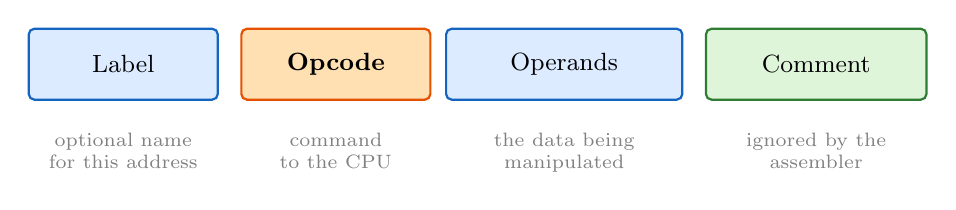
\begin{tikzpicture}[x=10mm, y=10mm]
        \node[blk,    minimum width=24mm] (lab) at (0,0)    {Label};
        \node[cpublk, minimum width=24mm] (op)  at (2.7,0)  {Opcode};
        \node[blk,    minimum width=30mm] (opd) at (5.6,0)  {Operands};
        \node[memblk, minimum width=28mm] (com) at (8.8,0)  {Comment};
        \node[lbl, anchor=north, align=center] at (0,-0.75)   {optional name\\for this address};
        \node[lbl, anchor=north, align=center] at (2.7,-0.75) {command\\to the CPU};
        \node[lbl, anchor=north, align=center] at (5.6,-0.75) {the data being\\manipulated};
        \node[lbl, anchor=north, align=center] at (8.8,-0.75) {ignored by the\\assembler};
    \end{tikzpicture}
    \end{center}

    \vspace{4mm}
    \begin{center}
    \begin{lstlisting}[style=armasm]
HERE    ADD     R1, R1, R0    ; add R0 to R1
    \end{lstlisting}
    \end{center}

    \vspace{3mm}
    {\small The \alert{first operand is the destination}. \texttt{ADD R1, R1, R0}
    means ``R1 becomes R1 plus R0.'' Read it from right to left.}

    \vspace{2mm}
    {\small \textbf{Directives} (\texttt{AREA}, \texttt{DCD}, \texttt{EQU},
    \texttt{ENTRY}, \texttt{END}) are commands to the \alert{assembler}.
    They generate no machine code. \textbf{Instructions} are commands to
    the \alert{processor}.}
\end{frame}

%===============================================================================
\section{The Load-Store Workflow}
%===============================================================================

\begin{frame}[plain]{Load, Process, Store}
    \begin{center}
    \includegraphics[width=.72\textwidth, height=.56\textheight, keepaspectratio]%
        {assets/loadstore-ops.pdf}
    \end{center}

    \vspace{2mm}
    {\small\centering Every operation on a memory variable follows the
    same three steps. No instruction can add two memory locations
    directly.\par}
\end{frame}

\begin{frame}[fragile]{The Workflow, in Instructions}
    \begin{columns}[T]
    \begin{column}{.44\textwidth}
        \textbf{In C}

        \vspace{1mm}
        {\ttfamily\normalsize counter = counter + 1;}

        \vspace{4mm}
        \textbf{What it must become}
        {\small
        \begin{enumerate}\itemsep1pt
            \item \alert{Load} the value into a register
            \item \alert{Process} it in the ALU
            \item \alert{Store} it back
        \end{enumerate}}
    \end{column}
    \begin{column}{.52\textwidth}
        \textbf{In assembly}

        \vspace{1mm}
        \begin{lstlisting}[style=armasm, basicstyle=\footnotesize\ttfamily]
	LDR  R1, =counter   ; address of counter
	LDR  R0, [R1]       ; load its value
	ADD  R0, R0, #1     ; add one
	STR  R0, [R1]       ; store it back
        \end{lstlisting}

        \vspace{3mm}
        {\small Notice the two different \texttt{LDR}s: \texttt{=counter}
        loads the \alert{address}. \texttt{[R1]} loads the \alert{value}
        at that address.}
    \end{column}
    \end{columns}

    \vspace{3mm}
    \begin{block}{Why one C statement becomes four instructions}
        This is the load-store principle from Chapter 2. Here you see
        its real cost. This is not inefficiency. It is what keeps the
        clock fast and the timing predictable.
    \end{block}
\end{frame}

%===============================================================================
\section{Load and Store Instructions}
%===============================================================================

\begin{frame}{The Load and Store Family}
	\begin{center}
		{\small
			\striped
			\begin{tabular}{@{}l l R{.50\textwidth}@{}}
				\toprule
				\textbf{Instruction} & \textbf{Size} & \textbf{Purpose} \\
				\midrule
				\texttt{LDR} / \texttt{STR}   & word     & Transfer 32 bits \\
				\texttt{LDRB} / \texttt{STRB} & byte     & Transfer 8 bits \\
				\texttt{LDRH} / \texttt{STRH} & halfword & Transfer 16 bits \\
				\texttt{LDRSB}                & byte     & Load byte and sign-extend \\
				\texttt{LDRSH}                & halfword & Load halfword and sign-extend \\
				\bottomrule
		\end{tabular}}
	\end{center}

	\vspace{3mm}

	\begin{block}{Naming convention}
		No suffix means a 32-bit \alert{word}.
		\texttt{B} means \alert{byte} (8 bits).
		\texttt{H} means \alert{halfword} (16 bits).
	\end{block}
\end{frame}

\begin{frame}{Load Group of Instructions}
	\begin{itemize}
		\item An LDR-type instruction fetches data from memory and puts
		the value into the destination register, \texttt{Rd}.
		\item Syntax: \\ %\verb|LDR Rd, [Rn, #offset]|
		\begin{center}
			{\ttfamily\normalsize
				\begin{tabular}{@{}l l@{}}
					LDR  Rd, [Rn, \#offset] \\
			\end{tabular}}
			\vspace{3mm}
		\end{center}
		\begin{itemize}
			\item \texttt{Rd}: destination register, where the loaded value is stored
			\item \texttt{Rn}: base register, holding the memory address
			\item \texttt{\#offset}: optional offset, added to the base register to compute the memory address
		\end{itemize}
	\end{itemize}
\end{frame}


\begin{frame}[fragile]{LDR: Loading a Word from Memory (Little-Endian)}
\begin{verbatim}
	LDR  R0, [R1]    ; load word
\end{verbatim}

	\centering
\resizebox{0.92\textwidth}{!}{%
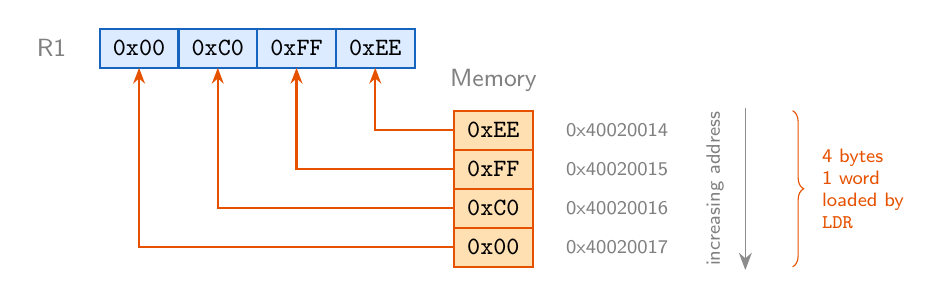
\begin{tikzpicture}[x=10mm, y=8mm]

	\def\bw{1.0}    % width of one byte box
	\def\rh{0.62}   % row height (matches the stack-frame diagram)

	% --- Register R1: four contiguous byte boxes ---
	\def\regx{0.7}
	\def\regy{4.3}
	\foreach \i/\val in {0/{0x00},1/{0xC0},2/{0xFF},3/{0xEE}}{
		\pgfmathsetmacro{\x}{\regx+\i*\bw}
		\draw[draw=blkline, fill=blkfill, thick]
		(\x,\regy) rectangle ({\x+\bw},{\regy-\rh});
		\node[font=\ttfamily\small] at ({\x+\bw/2},{\regy-\rh/2}) {\val};
	}
	\node[lbl, anchor=east, font=\sffamily\small] at ({\regx-0.3},{\regy-\rh/2}) {R1};

	% --- Memory: four stacked byte boxes, addresses increasing downward ---
	\def\memx{5.2}
	\def\memy{3.0}
	\foreach \i/\val/\addr in {%
		0/{0xEE}/{0x40020014},
		1/{0xFF}/{0x40020015},
		2/{0xC0}/{0x40020016},
		3/{0x00}/{0x40020017}}{
		\pgfmathsetmacro{\y}{\memy-\i*\rh}
		\draw[draw=accentline, fill=accentfill, thick]
		(\memx,\y) rectangle ({\memx+\bw},{\y-\rh});
		\node[font=\ttfamily\small] at ({\memx+\bw/2},{\y-\rh/2}) {\val};
		\node[lbl, anchor=west, font=\sffamily\scriptsize] at ({\memx+\bw+0.3},{\y-\rh/2}) {\addr};
	}
	\node[lbl, anchor=south, font=\sffamily\small] at ({\memx+\bw/2},{\memy+0.15}) {Memory};

	% --- Arrows: bytes flow up from memory into the register (LDR) ---
	\draw[flow, draw=accentline] (\memx,{\memy-0*\rh-\rh/2}) -| ({\regx+3*\bw+\bw/2},{\regy-\rh});
	\draw[flow, draw=accentline] (\memx,{\memy-1*\rh-\rh/2}) -| ({\regx+2*\bw+\bw/2},{\regy-\rh});
	\draw[flow, draw=accentline] (\memx,{\memy-2*\rh-\rh/2}) -| ({\regx+1*\bw+\bw/2},{\regy-\rh});
	\draw[flow, draw=accentline] (\memx,{\memy-3*\rh-\rh/2}) -| ({\regx+0*\bw+\bw/2},{\regy-\rh});

	% --- Address axis, to the right of the address column ---
	\def\axisx{8.9}
	\draw[-{Stealth[length=2.2mm]}, draw=black!45]
	({\axisx},{\memy+0.05}) -- ({\axisx},{\memy-4*\rh-0.05});
	\node[lbl, anchor=south, rotate=90, font=\sffamily\scriptsize]
	at ({\axisx-0.15},{\memy-2*\rh}) {increasing address};

	% --- Brace naming the whole word ---
	\draw[decorate, decoration={brace, amplitude=4pt}, draw=accentline]
	({\axisx+0.6},{\memy}) -- ({\axisx+0.6},{\memy-4*\rh});
	\node[lbl, anchor=west, align=left, font=\sffamily\scriptsize, text=accentline]
	at ({\axisx+0.85},{\memy-2*\rh}) {4 bytes\\1 word\\loaded by\\\texttt{LDR}};

\end{tikzpicture}%\
}
	\begin{itemize}
	\item Assume R0 = 0x40020014, and the \alert{memory word} at 0x40020014 holds 0x00C0FFEE.
	\item After \texttt{LDR R1, [R0]} runs, the destination register R1 holds 0x00C0FFEE.
\end{itemize}

\end{frame}

\begin{frame}[fragile]{Choosing the Correct Data Width}
	\begin{center}
	\begin{lstlisting}[style=armasm]
		LDR   R0, [R1]    ; load 32 bits
		LDRH  R0, [R1]    ; load 16 bits (H = halfword)
		LDRB  R0, [R1]    ; load 8 bits (B = byte)
		LDRSH R0, [R1]    ; load 16 bits (SH = signed halfword)
		LDRSB R0, [R1]    ; load 8 bits (SB = signed byte)
	\end{lstlisting}
	\end{center}

	\vspace{3mm}

	\begin{block}{A register is always 32 bits wide}
		When fewer than 32 bits are loaded, the processor must decide
		what fills the unused upper bits. This gives two important ideas:
		\alert{zero extension} and \alert{sign extension}.
	\end{block}
\end{frame}

\begin{frame}[plain]{Zero Extension}{\texttt{LDRB} and \texttt{LDRH}}
	\begin{center}
		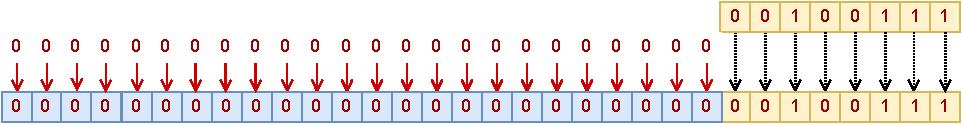
\includegraphics[width=.8\textwidth]{assets/bits-ldrb.pdf}

		\vspace{4mm}

		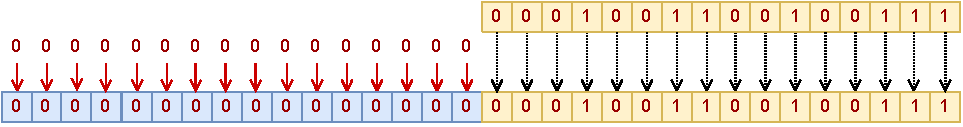
\includegraphics[width=.8\textwidth]{assets/bits-ldrh.pdf}
	\end{center}

	\vspace{3mm}

	{\small\centering
		The loaded value is treated as \textbf{unsigned}. Every unused
		upper bit is set to zero.\par}
\end{frame}

\begin{frame}[plain]{Sign Extension}{\texttt{LDRSB} and \texttt{LDRSH}}
	\begin{center}
		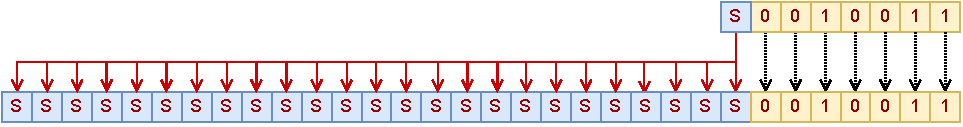
\includegraphics[width=.8\textwidth]{assets/bits-ldrsb.pdf}

		\vspace{4mm}

		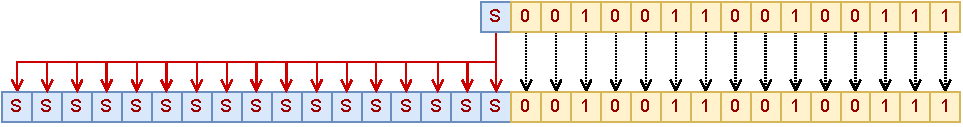
\includegraphics[width=.8\textwidth]{assets/bits-ldrsh.pdf}
	\end{center}

	\vspace{3mm}

	{\small\centering
		The sign bit is copied into all higher bits. This keeps the
		loaded value's signed meaning the same, even after it becomes
		32 bits wide.\par}
\end{frame}

% \bw, \rh shared by every frame
\def\bw{1.0}
\def\rh{0.62}
\def\regx{0.7}
\def\regy{4.3}
\def\memx{5.2}
\def\memy{3.0}


\begin{frame}[fragile]{LDRH Instruction}
\begin{verbatim}
	LDRH  R0, [R1]    ; load halfword
\end{verbatim}
\resizebox{0.92\textwidth}{!}{%
	\begin{tikzpicture}[x=10mm, y=8mm]

		% --- Register R1: byte3..byte0 left to right; only byte1,byte0 loaded ---
		\foreach \p/\val/\loaded in {0/{0x00}/0, 1/{0x00}/0, 2/{0xFF}/1, 3/{0xEE}/1}{
			\pgfmathsetmacro{\x}{\regx+\p*\bw}
			\ifnum\loaded=1
			\draw[loadedbox] (\x,\regy) rectangle ({\x+\bw},{\regy-\rh});
			\else
			\draw[extbox] (\x,\regy) rectangle ({\x+\bw},{\regy-\rh});
			\fi
			\node[font=\ttfamily\small] at ({\x+\bw/2},{\regy-\rh/2}) {\val};
		}
		\node[lbl, anchor=east, font=\sffamily\small] at ({\regx-0.3},{\regy-\rh/2}) {R1};

		% under-brace: zero-extended upper half
		\draw[decorate, decoration={brace, amplitude=4pt, mirror}, draw=blkline]
		({\regx},{\regy-\rh-0.1}) -- ({\regx+2*\bw},{\regy-\rh-0.1});
		\node[lbl, font=\sffamily\scriptsize, text=blkline, align=center]
		at ({\regx+\bw},{\regy-\rh-0.7}) {bits 31:16 = 0\\(zero-extended)};

		% --- Memory: 2 bytes, low address on top (LSB) ---
			\foreach \i/\val/\addr/\written in {%
	0/{0xEE}/{0x40020014}/1,
	1/{0xFF}/{0x40020015}/1,
	2/{0xC0}/{0x40020016}/0,
	3/{0x00}/{0x40020017}/0}{
	\pgfmathsetmacro{\y}{\memy-\i*\rh}
	\ifnum\written=1
	\draw[memwrite] (\memx,\y) rectangle ({\memx+\bw},{\y-\rh});
	\else
	\draw[memkeep] (\memx,\y) rectangle ({\memx+\bw},{\y-\rh});
	\fi
	\node[font=\ttfamily\small] at ({\memx+\bw/2},{\y-\rh/2}) {\val};
	\node[lbl, anchor=west, font=\sffamily\scriptsize] at ({\memx+\bw+0.3},{\y-\rh/2}) {\addr};
	}
	\node[lbl, anchor=south, font=\sffamily\small] at ({\memx+\bw/2},{\memy+0.15}) {Memory};

		% --- Arrows: 2 bytes flow up into byte1,byte0 ---
		\draw[flow, draw=accentline] (\memx,{\memy-0*\rh-\rh/2}) -| ({\regx+3*\bw+\bw/2},{\regy-\rh});
		\draw[flow, draw=accentline] (\memx,{\memy-1*\rh-\rh/2}) -| ({\regx+2*\bw+\bw/2},{\regy-\rh});

		% --- Address axis + brace ---
		\def\axisx{9.1}
		\draw[-{Stealth[length=2.2mm]}, draw=black!45]
		({\axisx},{\memy+0.05}) -- ({\axisx},{\memy-2*\rh-0.05});
		\node[lbl, anchor=south, rotate=90, font=\sffamily\scriptsize]
		at ({\axisx-0.15},{\memy-1*\rh}) {increasing address};
		\draw[decorate, decoration={brace, amplitude=4pt}, draw=accentline]
		({\axisx+0.6},{\memy}) -- ({\axisx+0.6},{\memy-2*\rh});
		\node[lbl, anchor=west, align=left, font=\sffamily\scriptsize, text=accentline]
		at ({\axisx+0.85},{\memy-1*\rh}) {2 bytes\\loaded by\\\texttt{LDRH}};

					% under-brace: unchanged memory bytes
		\draw[decorate, decoration={brace, amplitude=4pt, mirror}, draw=accentline]
		({\memx-.1},{\memy-2*\rh}) -- ({\memx-.1},{\memy-4*\rh-0.1});
		\node[lbl, font=\sffamily\scriptsize, text=accentline, align=center]
		at ({\memx-\bw/2-.4},{\memy-2*\rh-0.7}) {not\\copied};

	\end{tikzpicture}%
}
	\vspace{4mm}

	\begin{itemize}
		\item Assume R0 = 0x40020014, and the \alert{memory halfword} at 0x40020014 holds 0xFFEE.
		\item After \texttt{LDRH R1, [R0]} runs, the lower halfword of R1 holds 0xFFEE, and the top halfword is \alert{cleared}.
	\end{itemize}
\end{frame}

\begin{frame}[fragile]{LDRB Instruction}
\resizebox{0.92\textwidth}{!}{%
	\begin{tikzpicture}[x=10mm, y=8mm]

		% --- Register R1: only byte0 loaded ---
		\foreach \p/\val/\loaded in {0/{0x00}/0, 1/{0x00}/0, 2/{0x00}/0, 3/{0xEE}/1}{
			\pgfmathsetmacro{\x}{\regx+\p*\bw}
			\ifnum\loaded=1
			\draw[loadedbox] (\x,\regy) rectangle ({\x+\bw},{\regy-\rh});
			\else
			\draw[extbox] (\x,\regy) rectangle ({\x+\bw},{\regy-\rh});
			\fi
			\node[font=\ttfamily\small] at ({\x+\bw/2},{\regy-\rh/2}) {\val};
		}
		\node[lbl, anchor=east, font=\sffamily\small] at ({\regx-0.3},{\regy-\rh/2}) {R1};

		% under-brace: zero-extended upper 3 bytes
		\draw[decorate, decoration={brace, amplitude=4pt, mirror}, draw=blkline]
		({\regx},{\regy-\rh-0.1}) -- ({\regx+3*\bw},{\regy-\rh-0.1});
		\node[lbl, font=\sffamily\scriptsize, text=blkline, align=center]
		at ({\regx+1.5*\bw},{\regy-\rh-0.7}) {bits 31:8 = 0\\(zero-extended)};

		% --- Memory: 1 byte ---
			% --- Memory: only the low byte overwritten, others keep their old value ---
\foreach \i/\val/\addr/\written in {%
	0/{0xEE}/{0x40020014}/1,
	1/{0xFF}/{0x40020015}/0,
	2/{0xC0}/{0x40020016}/0,
	3/{0x00}/{0x40020017}/0}{
	\pgfmathsetmacro{\y}{\memy-\i*\rh}
	\ifnum\written=1
	\draw[memwrite] (\memx,\y) rectangle ({\memx+\bw},{\y-\rh});
	\else
	\draw[memkeep] (\memx,\y) rectangle ({\memx+\bw},{\y-\rh});
	\fi
	\node[font=\ttfamily\small] at ({\memx+\bw/2},{\y-\rh/2}) {\val};
	\node[lbl, anchor=west, font=\sffamily\scriptsize] at ({\memx+\bw+0.3},{\y-\rh/2}) {\addr};
}
\node[lbl, anchor=south, font=\sffamily\small] at ({\memx+\bw/2},{\memy+0.15}) {Memory};

		% --- Arrow: 1 byte flows up into byte0 ---
		\draw[flow, draw=accentline] (\memx,{\memy-\rh/2}) -| ({\regx+3*\bw+\bw/2},{\regy-\rh});

		% --- Address axis + brace ---
		\def\axisx{9.1}
		\draw[-{Stealth[length=2.2mm]}, draw=black!45]
		({\axisx},{\memy+0.05}) -- ({\axisx},{\memy-\rh-0.05});
		\node[lbl, anchor=south, rotate=90, font=\sffamily\scriptsize]
		at ({\axisx-0.15},{\memy-0.5*\rh}) {addr.};
		\draw[decorate, decoration={brace, amplitude=4pt}, draw=accentline]
		({\axisx+0.6},{\memy}) -- ({\axisx+0.6},{\memy-\rh});
		\node[lbl, anchor=west, align=left, font=\sffamily\scriptsize, text=accentline]
		at ({\axisx+0.85},{\memy-0.5*\rh}) {1 byte\\loaded by\\\texttt{LDRB}};

			% under-brace: unchanged memory bytes
\draw[decorate, decoration={brace, amplitude=4pt, mirror}, draw=accentline]
({\memx-0.1},{\memy-1*\rh}) -- ({\memx-0.1},{\memy-4*\rh});
\node[lbl, font=\sffamily\scriptsize, text=accentline, align=center]
at ({\memx-\bw/2-.4},{\memy-2*\rh-0.35}) {not\\copied};

	\end{tikzpicture}%
}
	\vspace{4mm}

	\begin{itemize}
		\item Assume R0 = 0x40020014, and the \alert{memory byte} at 0x40020014 holds 0xEE.
		\item After \texttt{LDRB R1, [R0]} runs, the lowest byte of R1 holds 0xEE, and the remaining bytes are \alert{cleared}.
	\end{itemize}
\end{frame}

\section{Loading Signed Numbers}

\begin{frame}{The Same Bits Can Mean Different Numbers}
	\begin{itemize}
		\item Most microprocessor work uses unsigned numbers.
		\item Sometimes, signed numbers are necessary
	\end{itemize}
	\begin{center}
		{
			\striped
			\begin{tabular}{@{}l l l@{}}
				\toprule
				\textbf{Byte in memory} & \textbf{\texttt{LDRB}} & \textbf{\texttt{LDRSB}} \\
				\midrule
				\texttt{0x7F} & \texttt{0x0000007F} = 127  & \texttt{0x0000007F} = 127 \\
				\texttt{0xFF} & \texttt{0x000000FF} = 255  & \texttt{0xFFFFFFFF} = -1 \\
				\texttt{0x80} & \texttt{0x00000080} = 128  & \texttt{0xFFFFFF80} = -128 \\
				\bottomrule
		\end{tabular}}
	\end{center}

	\vspace{3mm}

	\begin{block}{The instruction states your \textbf{intent}}
		Memory only stores bits. Choosing \texttt{LDRB} or \texttt{LDRSB}
		tells the processor whether those bits mean an unsigned value or
		a signed one.
	\end{block}
\end{frame}

\begin{frame}[fragile]{LDRSH Instruction}
	\begin{verbatim}
	LDRSH R0, [R1]    ; load signed halfword
\end{verbatim}
\resizebox{0.92\textwidth}{!}{%
	\begin{tikzpicture}[x=10mm, y=8mm]

		% --- Register R1: byte1,byte0 loaded; byte3,byte2 replicate the sign bit ---
		\foreach \p/\val/\loaded in {0/{0xFF}/0, 1/{0xFF}/0, 2/{0xFF}/1, 3/{0xEE}/1}{
			\pgfmathsetmacro{\x}{\regx+\p*\bw}
			\ifnum\loaded=1
			\draw[loadedbox] (\x,\regy) rectangle ({\x+\bw},{\regy-\rh});
			\else
			\draw[extbox] (\x,\regy) rectangle ({\x+\bw},{\regy-\rh});
			\fi
			\node[font=\ttfamily\small] at ({\x+\bw/2},{\regy-\rh/2}) {\val};
		}
		\node[lbl, anchor=east, font=\sffamily\small] at ({\regx-0.3},{\regy-\rh/2}) {R1};

		% under-brace: sign-extended upper half
		\draw[decorate, decoration={brace, amplitude=4pt, mirror}, draw=blkline]
		({\regx},{\regy-\rh-0.1}) -- ({\regx+2*\bw},{\regy-\rh-0.1});
		\node[lbl, font=\sffamily\scriptsize, text=blkline, align=center]
		at ({\regx+\bw},{\regy-\rh-0.7}) {bits 31:16 = bit 15\\(sign-extended)};

		% --- Memory: 2 bytes, same halfword 0xFF80 as LDRH (bit 15 = 1) ---
			\foreach \i/\val/\addr/\written in {%
	0/{0xEE}/{0x40020014}/1,
	1/{0xFF}/{0x40020015}/1,
	2/{0xC0}/{0x40020016}/0,
	3/{0x00}/{0x40020017}/0}{
	\pgfmathsetmacro{\y}{\memy-\i*\rh}
	\ifnum\written=1
	\draw[memwrite] (\memx,\y) rectangle ({\memx+\bw},{\y-\rh});
	\else
	\draw[memkeep] (\memx,\y) rectangle ({\memx+\bw},{\y-\rh});
	\fi
	\node[font=\ttfamily\small] at ({\memx+\bw/2},{\y-\rh/2}) {\val};
	\node[lbl, anchor=west, font=\sffamily\scriptsize] at ({\memx+\bw+0.3},{\y-\rh/2}) {\addr};
}
\node[lbl, anchor=south, font=\sffamily\small] at ({\memx+\bw/2},{\memy+0.15}) {Memory};

		% --- Arrows: 2 bytes flow up into byte1,byte0 ---
		\draw[flow, draw=accentline] (\memx,{\memy-0*\rh-\rh/2}) -| ({\regx+3*\bw+\bw/2},{\regy-\rh});
		\draw[flow, draw=accentline] (\memx,{\memy-1*\rh-\rh/2}) -| ({\regx+2*\bw+\bw/2},{\regy-\rh});

		% --- Address axis + brace ---
		\def\axisx{9.1}
		\draw[-{Stealth[length=2.2mm]}, draw=black!45]
		({\axisx},{\memy+0.05}) -- ({\axisx},{\memy-2*\rh-0.05});
		\node[lbl, anchor=south, rotate=90, font=\sffamily\scriptsize]
		at ({\axisx-0.15},{\memy-1*\rh}) {increasing address};
		\draw[decorate, decoration={brace, amplitude=4pt}, draw=accentline]
		({\axisx+0.6},{\memy}) -- ({\axisx+0.6},{\memy-2*\rh});
		\node[lbl, anchor=west, align=left, font=\sffamily\scriptsize, text=accentline]
		at ({\axisx+0.85},{\memy-1*\rh}) {2 bytes\\loaded by\\\texttt{LDRSH}};

			% under-brace: unchanged memory bytes
\draw[decorate, decoration={brace, amplitude=4pt, mirror}, draw=accentline]
({\memx-.1},{\memy-2*\rh}) -- ({\memx-.1},{\memy-4*\rh-0.1});
\node[lbl, font=\sffamily\scriptsize, text=accentline, align=center]
at ({\memx-\bw/2-.4},{\memy-2*\rh-0.7}) {not\\copied};

	\end{tikzpicture}%
}
	\vspace{4mm}

	\begin{itemize}
		\item Assume R0 = 0x40020014, and the \alert{memory halfword} at 0x40020014 holds 0xEEFF.
		\item After \texttt{LDRH R1, [R0]} runs, the lower halfword of R1 holds 0xFFEE, and the top halfword holds the sign bit of the loaded halfword.
	\end{itemize}
\end{frame}

\begin{frame}[fragile]{LDRSB Instruction}
	\begin{verbatim}
		LDRSB R0, [R1]    ; load signed byte
	\end{verbatim}
\resizebox{0.92\textwidth}{!}{%
	\begin{tikzpicture}[x=10mm, y=8mm]

		% --- Register R1: only byte0 loaded; byte3,byte2,byte1 replicate the sign bit ---
		\foreach \p/\val/\loaded in {0/{0xFF}/0, 1/{0xFF}/0, 2/{0xFF}/0, 3/{0xEE}/1}{
			\pgfmathsetmacro{\x}{\regx+\p*\bw}
			\ifnum\loaded=1
			\draw[loadedbox] (\x,\regy) rectangle ({\x+\bw},{\regy-\rh});
			\else
			\draw[extbox] (\x,\regy) rectangle ({\x+\bw},{\regy-\rh});
			\fi
			\node[font=\ttfamily\small] at ({\x+\bw/2},{\regy-\rh/2}) {\val};
		}
		\node[lbl, anchor=east, font=\sffamily\small] at ({\regx-0.3},{\regy-\rh/2}) {R1};

		% under-brace: sign-extended upper 3 bytes
		\draw[decorate, decoration={brace, amplitude=4pt, mirror}, draw=blkline]
		({\regx},{\regy-\rh-0.1}) -- ({\regx+3*\bw},{\regy-\rh-0.1});
		\node[lbl, font=\sffamily\scriptsize, text=blkline, align=center]
		at ({\regx+1.5*\bw},{\regy-\rh-0.7}) {bits 31:8 = bit 7\\(sign-extended)};

		% --- Memory: 1 byte, same source byte 0x80 as LDRB (bit 7 = 1) ---
\foreach \i/\val/\addr/\written in {%
	0/{0xEE}/{0x40020014}/1,
	1/{0xFF}/{0x40020015}/0,
	2/{0xC0}/{0x40020016}/0,
	3/{0x00}/{0x40020017}/0}{
	\pgfmathsetmacro{\y}{\memy-\i*\rh}
	\ifnum\written=1
	\draw[memwrite] (\memx,\y) rectangle ({\memx+\bw},{\y-\rh});
	\else
	\draw[memkeep] (\memx,\y) rectangle ({\memx+\bw},{\y-\rh});
	\fi
	\node[font=\ttfamily\small] at ({\memx+\bw/2},{\y-\rh/2}) {\val};
	\node[lbl, anchor=west, font=\sffamily\scriptsize] at ({\memx+\bw+0.3},{\y-\rh/2}) {\addr};
}
\node[lbl, anchor=south, font=\sffamily\small] at ({\memx+\bw/2},{\memy+0.15}) {Memory};

		% --- Arrow: 1 byte flows up into byte0 ---
		\draw[flow, draw=accentline] (\memx,{\memy-\rh/2}) -| ({\regx+3*\bw+\bw/2},{\regy-\rh});

		% --- Address axis + brace ---
		\def\axisx{9.1}
		\draw[-{Stealth[length=2.2mm]}, draw=black!45]
		({\axisx},{\memy+0.05}) -- ({\axisx},{\memy-\rh-0.05});
		\node[lbl, anchor=south, rotate=90, font=\sffamily\scriptsize]
		at ({\axisx-0.15},{\memy-0.5*\rh}) {addr.};
		\draw[decorate, decoration={brace, amplitude=4pt}, draw=accentline]
		({\axisx+0.6},{\memy}) -- ({\axisx+0.6},{\memy-\rh});
		\node[lbl, anchor=west, align=left, font=\sffamily\scriptsize, text=accentline]
		at ({\axisx+0.85},{\memy-0.5*\rh}) {1 byte\\loaded by\\\texttt{LDRSB}};

			% under-brace: unchanged memory bytes
\draw[decorate, decoration={brace, amplitude=4pt, mirror}, draw=accentline]
({\memx-0.1},{\memy-1*\rh}) -- ({\memx-0.1},{\memy-4*\rh});
\node[lbl, font=\sffamily\scriptsize, text=accentline, align=center]
at ({\memx-\bw/2-.4},{\memy-2*\rh-0.35}) {not\\copied};


	\end{tikzpicture}%
}
	\vspace{4mm}

	\begin{itemize}
		\item Assume R0 = 0x40020014, and the \alert{memory byte} at 0x40020014 holds 0xEE.
		\item After \texttt{LDRSB R1, [R0]} runs, the lowest byte of R1 holds 0xEE, and the remaining bytes hold the sign bit of the loaded byte.
	\end{itemize}
\end{frame}

\section{Store Instructions}

% ==================================================================
% STR — store a full word
% ==================================================================
\begin{frame}[fragile]{STR: Storing a Word to Memory}
	\begin{verbatim}
	STR   R0, [R1]    ; store 32-bit word
	\end{verbatim}
	\centering
	{\small\itshape Before: R1 = 0x11223344, \quad [0x40020014] = 0x00C0FFEE\par}
	\vspace{2mm}
	\resizebox{0.92\textwidth}{!}{%
		\begin{tikzpicture}[x=10mm, y=8mm]

			% --- Register R1: all four bytes are stored ---
			\foreach \p/\val in {0/{0x11}, 1/{0x22}, 2/{0x33}, 3/{0x44}}{
				\pgfmathsetmacro{\x}{\regx+\p*\bw}
				\draw[loadedbox] (\x,\regy) rectangle ({\x+\bw},{\regy-\rh});
				\node[font=\ttfamily\small] at ({\x+\bw/2},{\regy-\rh/2}) {\val};
			}
			\node[lbl, anchor=east, font=\sffamily\small] at ({\regx-0.3},{\regy-\rh/2}) {R1};

			% --- Memory: all four bytes overwritten, low address on top (LSB) ---
			\foreach \i/\val/\addr in {%
				0/{0x44}/{0x40020014},
				1/{0x33}/{0x40020015},
				2/{0x22}/{0x40020016},
				3/{0x11}/{0x40020017}}{
				\pgfmathsetmacro{\y}{\memy-\i*\rh}
				\draw[memwrite] (\memx,\y) rectangle ({\memx+\bw},{\y-\rh});
				\node[font=\ttfamily\small] at ({\memx+\bw/2},{\y-\rh/2}) {\val};
				\node[lbl, anchor=west, font=\sffamily\scriptsize] at ({\memx+\bw+0.3},{\y-\rh/2}) {\addr};
			}
			\node[lbl, anchor=south, font=\sffamily\small] at ({\memx+\bw/2},{\memy+0.15}) {Memory};

			% --- Arrows: all four bytes flow down from register into memory ---
			\draw[flow, draw=blkline] ({\regx+3*\bw+\bw/2},{\regy-\rh}) |- (\memx,{\memy-0*\rh-\rh/2});
			\draw[flow, draw=blkline] ({\regx+2*\bw+\bw/2},{\regy-\rh}) |- (\memx,{\memy-1*\rh-\rh/2});
			\draw[flow, draw=blkline] ({\regx+1*\bw+\bw/2},{\regy-\rh}) |- (\memx,{\memy-2*\rh-\rh/2});
			\draw[flow, draw=blkline] ({\regx+0*\bw+\bw/2},{\regy-\rh}) |- (\memx,{\memy-3*\rh-\rh/2});

			% --- Address axis + brace ---
			\def\axisx{9.1}
			\draw[-{Stealth[length=2.2mm]}, draw=black!45]
			({\axisx},{\memy+0.05}) -- ({\axisx},{\memy-4*\rh-0.05});
			\node[lbl, anchor=south, rotate=90, font=\sffamily\scriptsize]
			at ({\axisx-0.15},{\memy-2*\rh}) {increasing address};
			\draw[decorate, decoration={brace, amplitude=4pt}, draw=accentline]
			({\axisx+0.6},{\memy}) -- ({\axisx+0.6},{\memy-4*\rh});
			\node[lbl, anchor=west, align=left, font=\sffamily\scriptsize, text=accentline]
			at ({\axisx+0.85},{\memy-2*\rh}) {4 bytes\\written by\\\texttt{STR}\\(old value\\is lost)};

		\end{tikzpicture}%
	}
\end{frame}


% ==================================================================
% STRH — store the low halfword only
% ==================================================================
\begin{frame}[fragile]{STRH: Storing a Halfword to Memory}
	\begin{verbatim}
		STRH R0, [R1]
	\end{verbatim}
	\centering
	{\small\itshape Before: R1 = 0x11223344, \quad [0x40020014] = 0x00C0FFEE\par}
	\vspace{2mm}
	\resizebox{0.92\textwidth}{!}{%
		\begin{tikzpicture}[x=10mm, y=8mm]

			% --- Register R1: only byte1,byte0 (low halfword) are stored ---
			\foreach \p/\val/\used in {0/{0x11}/0, 1/{0x22}/0, 2/{0x33}/1, 3/{0x44}/1}{
				\pgfmathsetmacro{\x}{\regx+\p*\bw}
				\ifnum\used=1
				\draw[loadedbox] (\x,\regy) rectangle ({\x+\bw},{\regy-\rh});
				\else
				\draw[extbox] (\x,\regy) rectangle ({\x+\bw},{\regy-\rh});
				\fi
				\node[font=\ttfamily\small] at ({\x+\bw/2},{\regy-\rh/2}) {\val};
			}
			\node[lbl, anchor=east, font=\sffamily\small] at ({\regx-0.3},{\regy-\rh/2}) {R1};

			% under-brace: high halfword not stored
			\draw[decorate, decoration={brace, amplitude=4pt, mirror}, draw=blkline]
			({\regx},{\regy-\rh-0.1}) -- ({\regx+2*\bw},{\regy-\rh-0.1});
			\node[lbl, font=\sffamily\scriptsize, text=blkline, align=center]
			at ({\regx+\bw},{\regy-\rh-0.55}) {bits 31:16\\(not stored)};

			% --- Memory: low 2 bytes overwritten, high 2 bytes keep their old value ---
			\foreach \i/\val/\addr/\written in {%
				0/{0x44}/{0x40020014}/1,
				1/{0x33}/{0x40020015}/1,
				2/{0xC0}/{0x40020016}/0,
				3/{0x00}/{0x40020017}/0}{
				\pgfmathsetmacro{\y}{\memy-\i*\rh}
				\ifnum\written=1
				\draw[memwrite] (\memx,\y) rectangle ({\memx+\bw},{\y-\rh});
				\else
				\draw[memkeep] (\memx,\y) rectangle ({\memx+\bw},{\y-\rh});
				\fi
				\node[font=\ttfamily\small] at ({\memx+\bw/2},{\y-\rh/2}) {\val};
				\node[lbl, anchor=west, font=\sffamily\scriptsize] at ({\memx+\bw+0.3},{\y-\rh/2}) {\addr};
			}
			\node[lbl, anchor=south, font=\sffamily\small] at ({\memx+\bw/2},{\memy+0.15}) {Memory};

			% under-brace: unchanged memory bytes
			\draw[decorate, decoration={brace, amplitude=4pt, mirror}, draw=accentline]
			({\memx-.1},{\memy-2*\rh}) -- ({\memx-.1},{\memy-4*\rh-0.1});
			\node[lbl, font=\sffamily\scriptsize, text=accentline, align=center]
			at ({\memx-\bw/2-.4},{\memy-2*\rh-0.5}) {unchanged};

			% --- Arrows: 2 bytes flow down from register into memory ---
			\draw[flow, draw=blkline] ({\regx+3*\bw+\bw/2},{\regy-\rh}) |- (\memx,{\memy-0*\rh-\rh/2});
			\draw[flow, draw=blkline] ({\regx+2*\bw+\bw/2},{\regy-\rh}) |- (\memx,{\memy-1*\rh-\rh/2});

			% --- Address axis + brace ---
			\def\axisx{9.1}
			\draw[-{Stealth[length=2.2mm]}, draw=black!45]
			({\axisx},{\memy+0.05}) -- ({\axisx},{\memy-4*\rh-0.05});
			\node[lbl, anchor=south, rotate=90, font=\sffamily\scriptsize]
			at ({\axisx-0.15},{\memy-2*\rh}) {increasing address};
			\draw[decorate, decoration={brace, amplitude=4pt}, draw=accentline]
			({\axisx+0.6},{\memy}) -- ({\axisx+0.6},{\memy-2*\rh});
			\node[lbl, anchor=west, align=left, font=\sffamily\scriptsize, text=accentline]
			at ({\axisx+0.85},{\memy-1*\rh}) {2 bytes\\written by\\\texttt{STRH}};

		\end{tikzpicture}%
	}
	\begin{itemize}
	\item Assume R0 = 0x40020014, R1 = 0x11223344.
	\item After \texttt{STRH R1, [R0]} runs, the \alert{memory halfword} at 0x40020014 holds 0x4433.
\end{itemize}
\end{frame}


% ==================================================================
% STRB — store a single byte
% ==================================================================
\begin{frame}[fragile]{STRB: Storing a Byte to Memory}
	\begin{verbatim}
	STRB R0, [R1]
\end{verbatim}
	\centering
	{\small\itshape Before: R1 = 0x11223344, \quad [0x40020014] = 0x00C0FFEE\par}
	\vspace{2mm}
	\resizebox{0.92\textwidth}{!}{%
		\begin{tikzpicture}[x=10mm, y=8mm]

			% --- Register R1: only byte0 (low byte) is stored ---
			\foreach \p/\val/\used in {0/{0x11}/0, 1/{0x22}/0, 2/{0x33}/0, 3/{0x44}/1}{
				\pgfmathsetmacro{\x}{\regx+\p*\bw}
				\ifnum\used=1
				\draw[loadedbox] (\x,\regy) rectangle ({\x+\bw},{\regy-\rh});
				\else
				\draw[extbox] (\x,\regy) rectangle ({\x+\bw},{\regy-\rh});
				\fi
				\node[font=\ttfamily\small] at ({\x+\bw/2},{\regy-\rh/2}) {\val};
			}
			\node[lbl, anchor=east, font=\sffamily\small] at ({\regx-0.3},{\regy-\rh/2}) {R1};

			% under-brace: upper 3 bytes not stored
			\draw[decorate, decoration={brace, amplitude=4pt, mirror}, draw=blkline]
			({\regx},{\regy-\rh-0.1}) -- ({\regx+3*\bw},{\regy-\rh-0.1});
			\node[lbl, font=\sffamily\scriptsize, text=blkline, align=center]
			at ({\regx+1.5*\bw},{\regy-\rh-0.55}) {bits 31:8\\(not stored)};

			% --- Memory: only the low byte overwritten, others keep their old value ---
			\foreach \i/\val/\addr/\written in {%
				0/{0x44}/{0x40020014}/1,
				1/{0xFF}/{0x40020015}/0,
				2/{0xC0}/{0x40020016}/0,
				3/{0x00}/{0x40020017}/0}{
				\pgfmathsetmacro{\y}{\memy-\i*\rh}
				\ifnum\written=1
				\draw[memwrite] (\memx,\y) rectangle ({\memx+\bw},{\y-\rh});
				\else
				\draw[memkeep] (\memx,\y) rectangle ({\memx+\bw},{\y-\rh});
				\fi
				\node[font=\ttfamily\small] at ({\memx+\bw/2},{\y-\rh/2}) {\val};
				\node[lbl, anchor=west, font=\sffamily\scriptsize] at ({\memx+\bw+0.3},{\y-\rh/2}) {\addr};
			}
			\node[lbl, anchor=south, font=\sffamily\small] at ({\memx+\bw/2},{\memy+0.15}) {Memory};

			% under-brace: unchanged memory bytes
			\draw[decorate, decoration={brace, amplitude=4pt, mirror}, draw=accentline]
			({\memx-0.1},{\memy-1*\rh}) -- ({\memx-0.1},{\memy-4*\rh});
			\node[lbl, font=\sffamily\scriptsize, text=accentline, align=center]
			at ({\memx-\bw/2-.4},{\memy-2*\rh-0.5}) {unchanged};

			% --- Arrow: 1 byte flows down from register into memory ---
			\draw[flow, draw=blkline] ({\regx+3*\bw+\bw/2},{\regy-\rh}) |- (\memx,{\memy-0*\rh-\rh/2});

			% --- Address axis + brace ---
			\def\axisx{9.1}
			\draw[-{Stealth[length=2.2mm]}, draw=black!45]
			({\axisx},{\memy+0.05}) -- ({\axisx},{\memy-4*\rh-0.05});
			\node[lbl, anchor=south, rotate=90, font=\sffamily\scriptsize]
			at ({\axisx-0.15},{\memy-2*\rh}) {increasing address};
			\draw[decorate, decoration={brace, amplitude=4pt}, draw=accentline]
			({\axisx+0.6},{\memy}) -- ({\axisx+0.6},{\memy-1*\rh});
			\node[lbl, anchor=west, align=left, font=\sffamily\scriptsize, text=accentline]
			at ({\axisx+0.85},{\memy-0.5*\rh}) {1 byte\\written by\\\texttt{STRB}};

		\end{tikzpicture}%
	}
	\begin{itemize}
	\item After \texttt{STRB R1, [R0]} runs, the \alert{memory byte} at 0x40020014 holds 0x44.
	\end{itemize}
\end{frame}


\begin{frame}[fragile]{Memory Copy Example}

\begin{lstlisting}[style=armasm, basicstyle=\normalsize\ttfamily]
	LDR R0, =0x2000
	LDR R1, =0x2004
	LDR R2, [R0]
	STR R2, [R1]
\end{lstlisting}

\vspace{10mm}


	\begin{columns}[T]

		% ============================== BEFORE ==============================
		\begin{column}{0.48\textwidth}
			\centering{\sffamily\bfseries Before}\\[1mm]
			\resizebox{\linewidth}{!}{%
				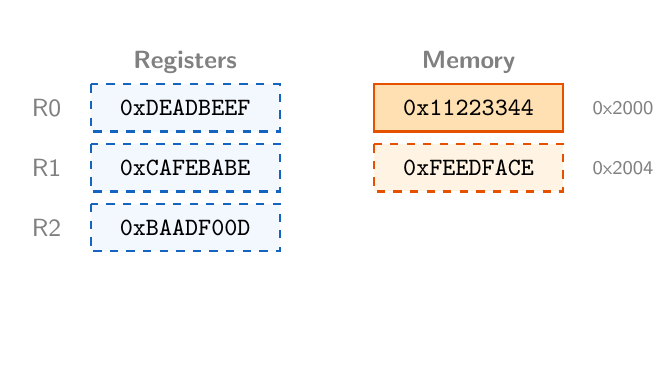
\begin{tikzpicture}[x=10mm, y=8mm]
					\path[use as bounding box] (-0.4,1.6) rectangle (7.4,6.9);

					\def\rw{2.4}
					\def\rh{0.75}
					\def\regx{0.4}
					\def\memx{4}
\def\rh{0.75} \def\rowsep{0.20} % desired gap
\def\rowA{6.0} \def\rowB{\rowA-\rh-\rowsep} \def\rowC{\rowB-\rh-\rowsep}

					\node[lbl, font=\sffamily\small\bfseries] at ({\regx+\rw/2},{\rowA+0.35}) {Registers};
					\node[lbl, font=\sffamily\small\bfseries] at ({\memx+\rw/2},{\rowA+0.35}) {Memory};

					\node[lbl, anchor=east, font=\sffamily\small] at ({\regx-0.25},{\rowA-\rh/2}) {R0};
					\draw[extbox] (\regx,\rowA) rectangle ({\regx+\rw},{\rowA-\rh});
					\node[font=\ttfamily\small] at ({\regx+\rw/2},{\rowA-\rh/2}) {0xDEADBEEF};

					\node[lbl, anchor=east, font=\sffamily\small] at ({\regx-0.25},{\rowB-\rh/2}) {R1};
					\draw[extbox] (\regx,\rowB) rectangle ({\regx+\rw},{\rowB-\rh});
					\node[font=\ttfamily\small] at ({\regx+\rw/2},{\rowB-\rh/2}) {0xCAFEBABE};

					\node[lbl, anchor=east, font=\sffamily\small] at ({\regx-0.25},{\rowC-\rh/2}) {R2};
					\draw[extbox] (\regx,\rowC) rectangle ({\regx+\rw},{\rowC-\rh});
					\node[font=\ttfamily\small] at ({\regx+\rw/2},{\rowC-\rh/2}) {0xBAADF00D};

					\node[lbl, anchor=west, font=\sffamily\scriptsize] at ({\memx+\rw+0.25},{\rowA-\rh/2}) {0x2000};
					\draw[memwrite] (\memx,\rowA) rectangle ({\memx+\rw},{\rowA-\rh});
					\node[font=\ttfamily\small] at ({\memx+\rw/2},{\rowA-\rh/2}) {0x11223344};

					\node[lbl, anchor=west, font=\sffamily\scriptsize] at ({\memx+\rw+0.25},{\rowB-\rh/2}) {0x2004};
					\draw[memkeep] (\memx,\rowB) rectangle ({\memx+\rw},{\rowB-\rh});
					\node[font=\ttfamily\small] at ({\memx+\rw/2},{\rowB-\rh/2}) {0xFEEDFACE};

				\end{tikzpicture}%
			}
		\end{column}

		% ============================== AFTER ===============================
		\begin{column}{0.48\textwidth}
			\centering{\sffamily\bfseries After}\\[1mm]
			\resizebox{\linewidth}{!}{%
				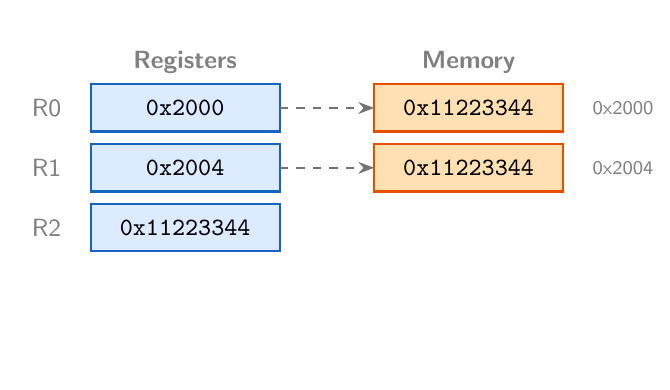
\begin{tikzpicture}[x=10mm, y=8mm]
					\path[use as bounding box] (-0.4,1.6) rectangle (7.4,6.9);

\def\rw{2.4}
\def\rh{0.75}
\def\regx{0.4}
\def\memx{4}
\def\rh{0.75} \def\rowsep{0.20} % desired gap
\def\rowA{6.0} \def\rowB{\rowA-\rh-\rowsep} \def\rowC{\rowB-\rh-\rowsep}

					\node[lbl, font=\sffamily\small\bfseries] at ({\regx+\rw/2},{\rowA+0.35}) {Registers};
					\node[lbl, font=\sffamily\small\bfseries] at ({\memx+\rw/2},{\rowA+0.35}) {Memory};

					\node[lbl, anchor=east, font=\sffamily\small] at ({\regx-0.25},{\rowA-\rh/2}) {R0};
					\draw[loadedbox] (\regx,\rowA) rectangle ({\regx+\rw},{\rowA-\rh});
					\node[font=\ttfamily\small] at ({\regx+\rw/2},{\rowA-\rh/2}) {0x2000};

					\node[lbl, anchor=east, font=\sffamily\small] at ({\regx-0.25},{\rowB-\rh/2}) {R1};
					\draw[loadedbox] (\regx,\rowB) rectangle ({\regx+\rw},{\rowB-\rh});
					\node[font=\ttfamily\small] at ({\regx+\rw/2},{\rowB-\rh/2}) {0x2004};

					\node[lbl, anchor=east, font=\sffamily\small] at ({\regx-0.25},{\rowC-\rh/2}) {R2};
					\draw[loadedbox] (\regx,\rowC) rectangle ({\regx+\rw},{\rowC-\rh});
					\node[font=\ttfamily\small] at ({\regx+\rw/2},{\rowC-\rh/2}) {0x11223344};

					\node[lbl, anchor=west, font=\sffamily\scriptsize] at ({\memx+\rw+0.25},{\rowA-\rh/2}) {0x2000};
					\draw[memwrite] (\memx,\rowA) rectangle ({\memx+\rw},{\rowA-\rh});
					\node[font=\ttfamily\small] at ({\memx+\rw/2},{\rowA-\rh/2}) {0x11223344};

					\node[lbl, anchor=west, font=\sffamily\scriptsize] at ({\memx+\rw+0.25},{\rowB-\rh/2}) {0x2004};
					\draw[memwrite] (\memx,\rowB) rectangle ({\memx+\rw},{\rowB-\rh});
					\node[font=\ttfamily\small] at ({\memx+\rw/2},{\rowB-\rh/2}) {0x11223344};

					% Address pointers, still true after execution (offset apart so both show)
					\draw[-{Stealth[length=2mm]}, dashed, draw=black!55, thick]
					({\regx+\rw},{\rowA-\rh/2}) -- ({\memx},{\rowA-\rh/2});
					\draw[-{Stealth[length=2mm]}, dashed, draw=black!55, thick]
					({\regx+\rw},{\rowB-\rh/2}) -- ({\memx},{\rowB-\rh/2});

				\end{tikzpicture}%
			}
		\end{column}

	\end{columns}

\vspace{1mm}
	{\scriptsize\color{black!55} dashed arrow = address used for addressing\par}

%	\begin{itemize}
%		\item \texttt{R0} and \texttt{R1} start out holding pointers to memory. We could have used \texttt{MOVW}/\texttt{MOVT} instead.
%		\item Square brackets always mean \alert{memory access}.
%	\end{itemize}

\end{frame}


%===============================================================================
\section{Registers in Practice}
%===============================================================================

\begin{frame}[plain]{Low and High Registers}
    \begin{columns}[c]
    \begin{column}{.46\textwidth}
        \begin{center}
        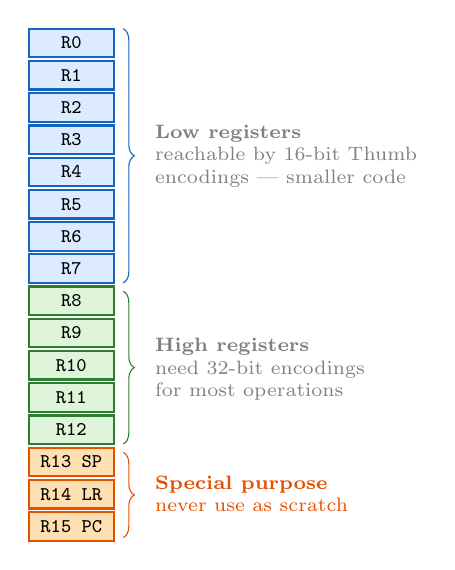
\begin{tikzpicture}[x=8mm, y=6.6mm]
        % Low registers R0-R7
        \foreach \i in {0,...,7}{
            \pgfmathsetmacro{\y}{-\i*0.62}
            \draw[draw=blkline, fill=blkfill, thick] (0,\y) rectangle (1.35,\y+0.55);
            \node[font=\scriptsize\ttfamily] at (0.675,\y+0.275) {R\i};
        }
        % High registers R8-R12
        \foreach \i in {8,...,12}{
            \pgfmathsetmacro{\y}{-(\i)*0.62}
            \draw[draw=memline, fill=memfill, thick] (0,\y) rectangle (1.35,\y+0.55);
            \node[font=\scriptsize\ttfamily] at (0.675,\y+0.275) {R\i};
        }
        % Special registers
        \foreach \i/\nm in {13/{R13 SP}, 14/{R14 LR}, 15/{R15 PC}}{
            \pgfmathsetmacro{\y}{-\i*0.62}
            \draw[draw=accentline, fill=accentfill, thick] (0,\y) rectangle (1.35,\y+0.55);
            \node[font=\scriptsize\ttfamily] at (0.675,\y+0.275) {\nm};
        }
        % Group braces and labels
        \draw[decorate, decoration={brace, amplitude=4pt}, draw=blkline]
            (1.5,0.55) -- (1.5,-4.34);
        \node[lbl, anchor=west, align=left, font=\scriptsize] at (1.85,-1.9)
            {\textbf{Low registers}\\{\scriptsize reachable by 16-bit Thumb}\\{\scriptsize encodings --- smaller code}};
        \draw[decorate, decoration={brace, amplitude=4pt}, draw=memline]
            (1.5,-4.5) -- (1.5,-7.44);
        \node[lbl, anchor=west, align=left, font=\scriptsize] at (1.85,-6.0)
            {\textbf{High registers}\\{\scriptsize need 32-bit encodings}\\{\scriptsize for most operations}};
        \draw[decorate, decoration={brace, amplitude=4pt}, draw=accentline]
            (1.5,-7.6) -- (1.5,-9.24);
        \node[lbl, anchor=west, align=left, font=\scriptsize, text=accentline] at (1.85,-8.4)
            {\textbf{Special purpose}\\{\scriptsize never use as scratch}};
        \end{tikzpicture}
        \end{center}
    \end{column}
    \begin{column}{.5\textwidth}
        {\small Preferring \texttt{R0}--\texttt{R7} is not just a style
        choice. It changes the size of the compiled program.}

        \vspace{3mm}
        \begin{block}{Seen in a disassembly}
            {\small \texttt{ADD R0, R1, R2} --- 16-bit Thumb\\
            \texttt{ADD R8, R9, R10} --- 32-bit Thumb-2}

            \vspace{1mm}
            {\small Same operation, but \alert{double} the flash footprint.}
        \end{block}

        \vspace{3mm}
        {\small \texttt{R13}/\texttt{R14}/\texttt{R15} keep their special
        meanings. Never use them as scratch storage.}
    \end{column}
    \end{columns}
\end{frame}

\begin{frame}[fragile]{Special Registers You Will See}
    \leavevmode
    {\small Three registers mean more than just ``a place to put a
    number.'' A disassembly window shows all three by name:}

    \vspace{2mm}
    \begin{center}
    {\small
    \striped
    \begin{tabular}{@{}l l R{.5\textwidth}@{}}
        \toprule
        \textbf{Register} & \textbf{Shown as} & \textbf{Role} \\
        \midrule
        R13 & \texttt{SP} & Stack pointer --- address of the last item pushed \\
        R14 & \texttt{LR} & Link register --- \texttt{BL} writes the return address here \\
        R15 & \texttt{PC} & Program counter --- writing it is a branch \\
        \bottomrule
    \end{tabular}}
    \end{center}

    \vspace{2mm}
    {\small The N/Z/C/V flags live in the \textbf{APSR}, part of the
    combined \texttt{xPSR}. This is often shown simply as \texttt{PSR}.
    Chapter 7 returns to these flags, once condition codes give them
    a use.}

    \vspace{2mm}
    \begin{block}{Prologue and epilogue}{Mark start and end of a function}
        \begin{lstlisting}[style=armasm, basicstyle=\normalsize\ttfamily]
	PUSH {LR}    ; save the return address
	...          ; the function body
	POP  {PC}    ; return by loading PC directly
        \end{lstlisting}
    \end{block}
\end{frame}

\begin{frame}{A Preview: Register Usage Conventions}
    \leavevmode
    {\small Two disassembly listings for the same C source always agree
    on \emph{which} registers carry arguments and results. This rule
    is called the \alert{AAPCS}.}

    \vspace{2mm}
    \begin{center}
    {\small
    \striped
    \begin{tabular}{@{}l R{.6\textwidth}@{}}
        \toprule
        \textbf{Registers} & \textbf{Role} \\
        \midrule
        \texttt{R0}--\texttt{R3} & First four arguments in; \texttt{R0} carries the return value out \\
        \texttt{R4}--\texttt{R11} & \emph{Callee-saved} --- a function may use them, but must restore them \\
        \bottomrule
    \end{tabular}}
    \end{center}

    \vspace{2mm}
    {\small This is why \texttt{scale()}, traced next, reads and writes
    \texttt{R0} with no register setup at all. The argument is already
    there.}

    \vspace{2mm}
    {\small Chapter 7 explains the full convention. Appendix B lists the
    complete standard.}
\end{frame}

%===============================================================================
\section{Constants and Addresses}
%===============================================================================

\begin{frame}[fragile]{\texttt{MOV} and \texttt{MVN}: Register-to-Register Data Movement}
	\leavevmode

	\begin{itemize}
		\item \texttt{MOV} copies a value into a register.
		\item The source can be another register or an encodable immediate.
		\item \texttt{MVN} performs the same operation after inverting every bit.
	\end{itemize}

	\vspace{2mm}

	\begin{center}
	\begin{lstlisting}[style=armasm]
	MOV R0, R1    ; copy R1 into R0
	MOV R0, #25   ; load decimal 25
	MVN R0, #0    ; R0 = 0xFFFFFFFF
	MVN R0, R1    ; R0 = ~R1
	\end{lstlisting}
	\end{center}

	\vspace{2mm}

	\begin{block}{What they cannot do}
	Neither instruction touches memory. Also, a single \texttt{MOV}
	cannot hold every possible 32-bit constant. So how do we load a
	large constant?
	\end{block}
\end{frame}

\begin{frame}[fragile]{Loading a Large Constant: \texttt{LDR Rd, =value}}
	\leavevmode
	\begin{center}
	\begin{lstlisting}[style=armasm, basicstyle=\large\ttfamily]
	LDR R0, =0x40020014
	\end{lstlisting}
	\end{center}
	\vspace{3mm}
	\begin{itemize}
		\item We often need constants that do not fit in a single \texttt{MOV} instruction.
		\item To avoid worrying about how it is encoded, we usually write \texttt{LDR Rd, =value}.
		\item This is an \alert{assembler pseudo-instruction}. It means:
	\end{itemize}
	\vspace{1mm}
	\begin{center} \textit{``Place this constant into the register.''} \end{center}
	\vspace{2mm}
	\begin{block}{Programmer versus assembler}
		You say \emph{what} value you want. The assembler decides
		\emph{how} to build it.
	\end{block}
\end{frame}

\begin{frame}[fragile]{How the Assembler Can Implement It}
	\leavevmode
	\begin{columns}[T]
	\begin{column}{.48\textwidth}
		\textbf{Option 1: Literal pool}

		\vspace{1mm}
		\begin{lstlisting}[style=armasm, basicstyle=\normalsize\ttfamily]
	LDR R0, [PC, #offset]
		\end{lstlisting}

		\vspace{5mm}
		The constant sits in memory. The processor loads it using a PC-relative address.
	\end{column}
	\begin{column}{.48\textwidth}
		\textbf{Option 2: Build it directly}

		\vspace{1mm}
		\begin{lstlisting}[style=armasm, basicstyle=\normalsize\ttfamily]
	MOVW R0, #0x0014
	MOVT R0, #0x4002
		\end{lstlisting}

		\vspace{5mm}
		The constant is built inside the register. No extra memory access is needed.
	\end{column}
	\end{columns}

	\vspace{3mm}
	\begin{block}{Key idea}
		\texttt{LDR Rd, =value} does not map to one specific machine
		instruction. It is just a request: put this constant into a
		register, however that is best done.
	\end{block}
\end{frame}

\begin{frame}[fragile]{Constructing a 32-Bit Constant with \texttt{MOVW}/\texttt{MOVT}}
	\leavevmode

	\begin{center}
	\begin{lstlisting}[style=armasm, basicstyle=\normalsize\ttfamily]
	MOVW R0, #0x0014   ; lower 16 bits
	MOVT R0, #0x4002   ; upper 16 bits
	\end{lstlisting}
	\end{center}

	\vspace{2mm}

	\begin{center}
		\large
		\texttt{R0 = 0x40020014}
	\end{center}

	\vspace{2mm}

\begin{block}{Why two instructions?}
A Thumb-2 instruction cannot hold just any 32-bit constant.\\ \texttt{MOVW} writes the lower half of the register. \texttt{MOVT} writes the upper half.
		\[
		\underbrace{\texttt{0x4002}}_{\text{upper 16 bits}}
		\quad
		\underbrace{\texttt{0x0014}}_{\text{lower 16 bits}}
		\]
	\end{block}
\end{frame}

\begin{frame}[fragile]{Reading Compiler Output}
	\leavevmode
	\begin{center}
	\begin{lstlisting}[style=armasm]
MOVW R3, #0x0014
MOVT R3, #0x4002
LDR  R2, [R3]
	\end{lstlisting}
	\end{center}

	\vspace{3mm}
	\begin{block}{How to read this sequence}
		Think of the first two instructions as one operation:
		\begin{center} \textit{``Build the address 0x40020014 in R3.''} \end{center}
		Once the address is in a register, the load can reach the
		memory-mapped peripheral register there.
	\end{block}
	\vspace{1mm}
	{\small In embedded programs, seeing a \texttt{MOVW}/\texttt{MOVT} pair usually means one address, or one large constant, is being built.}
\end{frame}

\begin{frame}{A Look Ahead: The Barrel Shifter}
    \leavevmode
    {\small ARM can shift a register on its way \emph{into} an
    instruction, at no extra cost --- for example \texttt{ADD R0, R1,
    R2, LSL \#2}. We will return to this feature in Chapter 6, where it
    becomes particularly useful for calculating addresses.}
\end{frame}

%===============================================================================
\section{Reading a Disassembly}
%===============================================================================

\begin{frame}[fragile]{Your First Disassembly}
    \begin{columns}[T]
    \begin{column}{.46\textwidth}
        \textbf{The listing}

        \vspace{1mm}
        \begin{lstlisting}[style=armasm]
	LDR  R3, [R7, #4]
	LDR  R2, [R7, #8]
	ADD  R3, R3, R2
	STR  R3, [R7, #12]
        \end{lstlisting}
    \end{column}
    \begin{column}{.5\textwidth}
        \textbf{Reading it back}
        {\small
        \begin{enumerate}\itemsep1pt
            \item \texttt{R7} is the \alert{frame pointer}, so these are
                  \alert{local variables} at offsets 4, 8, and 12
            \item Load two of them
            \item Add them
            \item Store the result in a third
        \end{enumerate}}

        \vspace{2mm}
        \textbf{The C was}

        \vspace{1mm}

        \begin{lstlisting}[style=myc]
	c = a + b;
	\end{lstlisting}

    %    {\ttfamily\normalsize c = a + b;}
    \end{column}
    \end{columns}

    \vspace{3mm}
    \begin{block}{Three things to notice}
        The whole statement follows \alert{load--process--store}. No
        \texttt{S} suffix appears, because nothing branches on the
        result. The offsets from \texttt{R7} tell you these are locals
        on the \alert{stack}, not global variables.
    \end{block}
\end{frame}

\begin{frame}{Summary}
    \begin{itemize}
        \item The goal is \textbf{literacy}, not fluency: enough to read a
              disassembly window and say what the processor is doing.
        \item A statement has four fields: \textbf{label}, \textbf{opcode},
              \textbf{operands}, \textbf{comment}. The first operand is the
              \textbf{destination}.
        \item Every operation on a memory variable follows
              \textbf{load--process--store}.
        \item \texttt{LDR Rn, =label} loads an \textbf{address}.
              \texttt{LDR Rn, [Rm]} loads a \textbf{value}.
        \item The suffix names the size: none $=$ \textbf{word}, \texttt{B} $=$
              \textbf{byte}, \texttt{H} $=$ \textbf{halfword}.
              \texttt{LDRB}/\texttt{LDRH} \textbf{zero-extend};
              \texttt{LDRSB}/\texttt{LDRSH} \textbf{sign-extend}.
        \item \textbf{Low registers} \texttt{R0}--\texttt{R7} are reachable by
              16-bit instructions, so compilers prefer them.
    \end{itemize}

    \vspace{2mm}
    \begin{block}{Next: Chapter 6 --- Memory, Arithmetic and Bit Manipulation}
        Next: how ARM calculates addresses efficiently, and the
        instructions that change individual bits.
    \end{block}
\end{frame}

%===============================================================================
\section{Design Challenge}
%===============================================================================

\begin{frame}{Design Challenge}{To be worked on paper, before any code}
    \leavevmode
    \begin{block}{The brief}
        A colleague's driver reads a 12-bit ADC result with
        \texttt{LDR} (a full word), then masks off the top 20 bits in
        C. Another engineer suggests using \texttt{LDRH} instead, since
        the ADC data register is only 16 bits wide.
    \end{block}

    \vspace{2mm}
    {\small Compare the two approaches instruction by instruction: how
    many instructions does each need, and does either risk reading
    memory that does not belong to the ADC register? Then consider a
    signed sensor reading stored as a 16-bit two's-complement value.
    Explain which load instruction is required, and what goes wrong if
    the wrong one is used. State the general rule you would give a
    junior engineer for choosing between \texttt{LDR}, \texttt{LDRH},
    and \texttt{LDRSH}.}
\end{frame}

\begin{frame}[plain]
    \begin{center}
        \vfill
        {\usebeamerfont{title}\color{primary}\Huge Questions?}
        \vfill
        {\small\color{Gray} \emph{Introduction to ARM Cortex-M Microprocessors} --- Chapter 5}
        \vfill
    \end{center}
\end{frame}

\end{document}
